The User Interface consists in a single page application, divided into three main views: the \textit{Request}, the \textit{Response} and the \textit{Map view}, as proposed in section \ref{sec:csa_design} and illustrated in figure \ref{fig:csa_tree}. Since the application is developed using React, every view is managed by a container, which reads the state from the store, calls the rendering of presentational components, and may dispatch actions on user input or other events. It is also worth nothing that, due to the modular nature of react components, they are reusable. This is particularly useful in the construction of the request view. As an example, one component (\textit{city form}) is used to collect information regarding all cities: origin, return city and cities to visit. This is possible because the underlying structure is the same. The only difference is the reference to these components, which update different parts of the state.  

\begin{figure}[htpb]
  \centering
  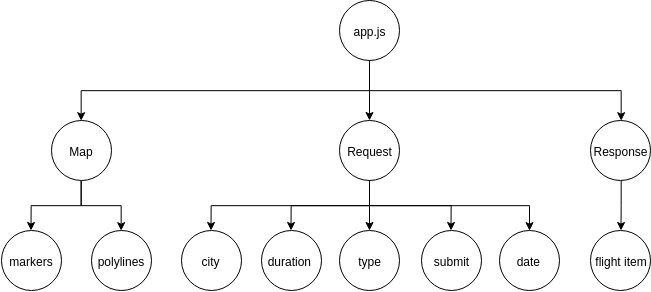
\includegraphics[width=.8\textwidth]{./Figures/system_implementation/csa_tree.png}
  \caption{Structure of the developed user interface}
  \label{fig:csa_tree}  
\end{figure}

The user interface was designed to be mobile friendly, by being responsive to the device size. This was achieved using the Bootstrap grid system, a web application design paradigm in which the user screen is divided into 12 columns, and each element of the user interface may specify a variable number of columns, depending on the screen size.

Figure \ref{fig:desktop_app} and \ref{fig:mobile_app} illustrate two possible views of the developed application. The first image illustrates the application in a desktop device and the second in a mobile. It is worth noting that these two screenshots correspond to the same application. The design differences between these two views is a result of the responsiveness of the application, which is responsible for resizing the application elements according to the device size. It also includes toggles in the \textit{Request} and \textit{Response} views, as to generate more space to the map view. 


\begin{figure}
\centering
\begin{minipage}{.7\textwidth}
  \centering
  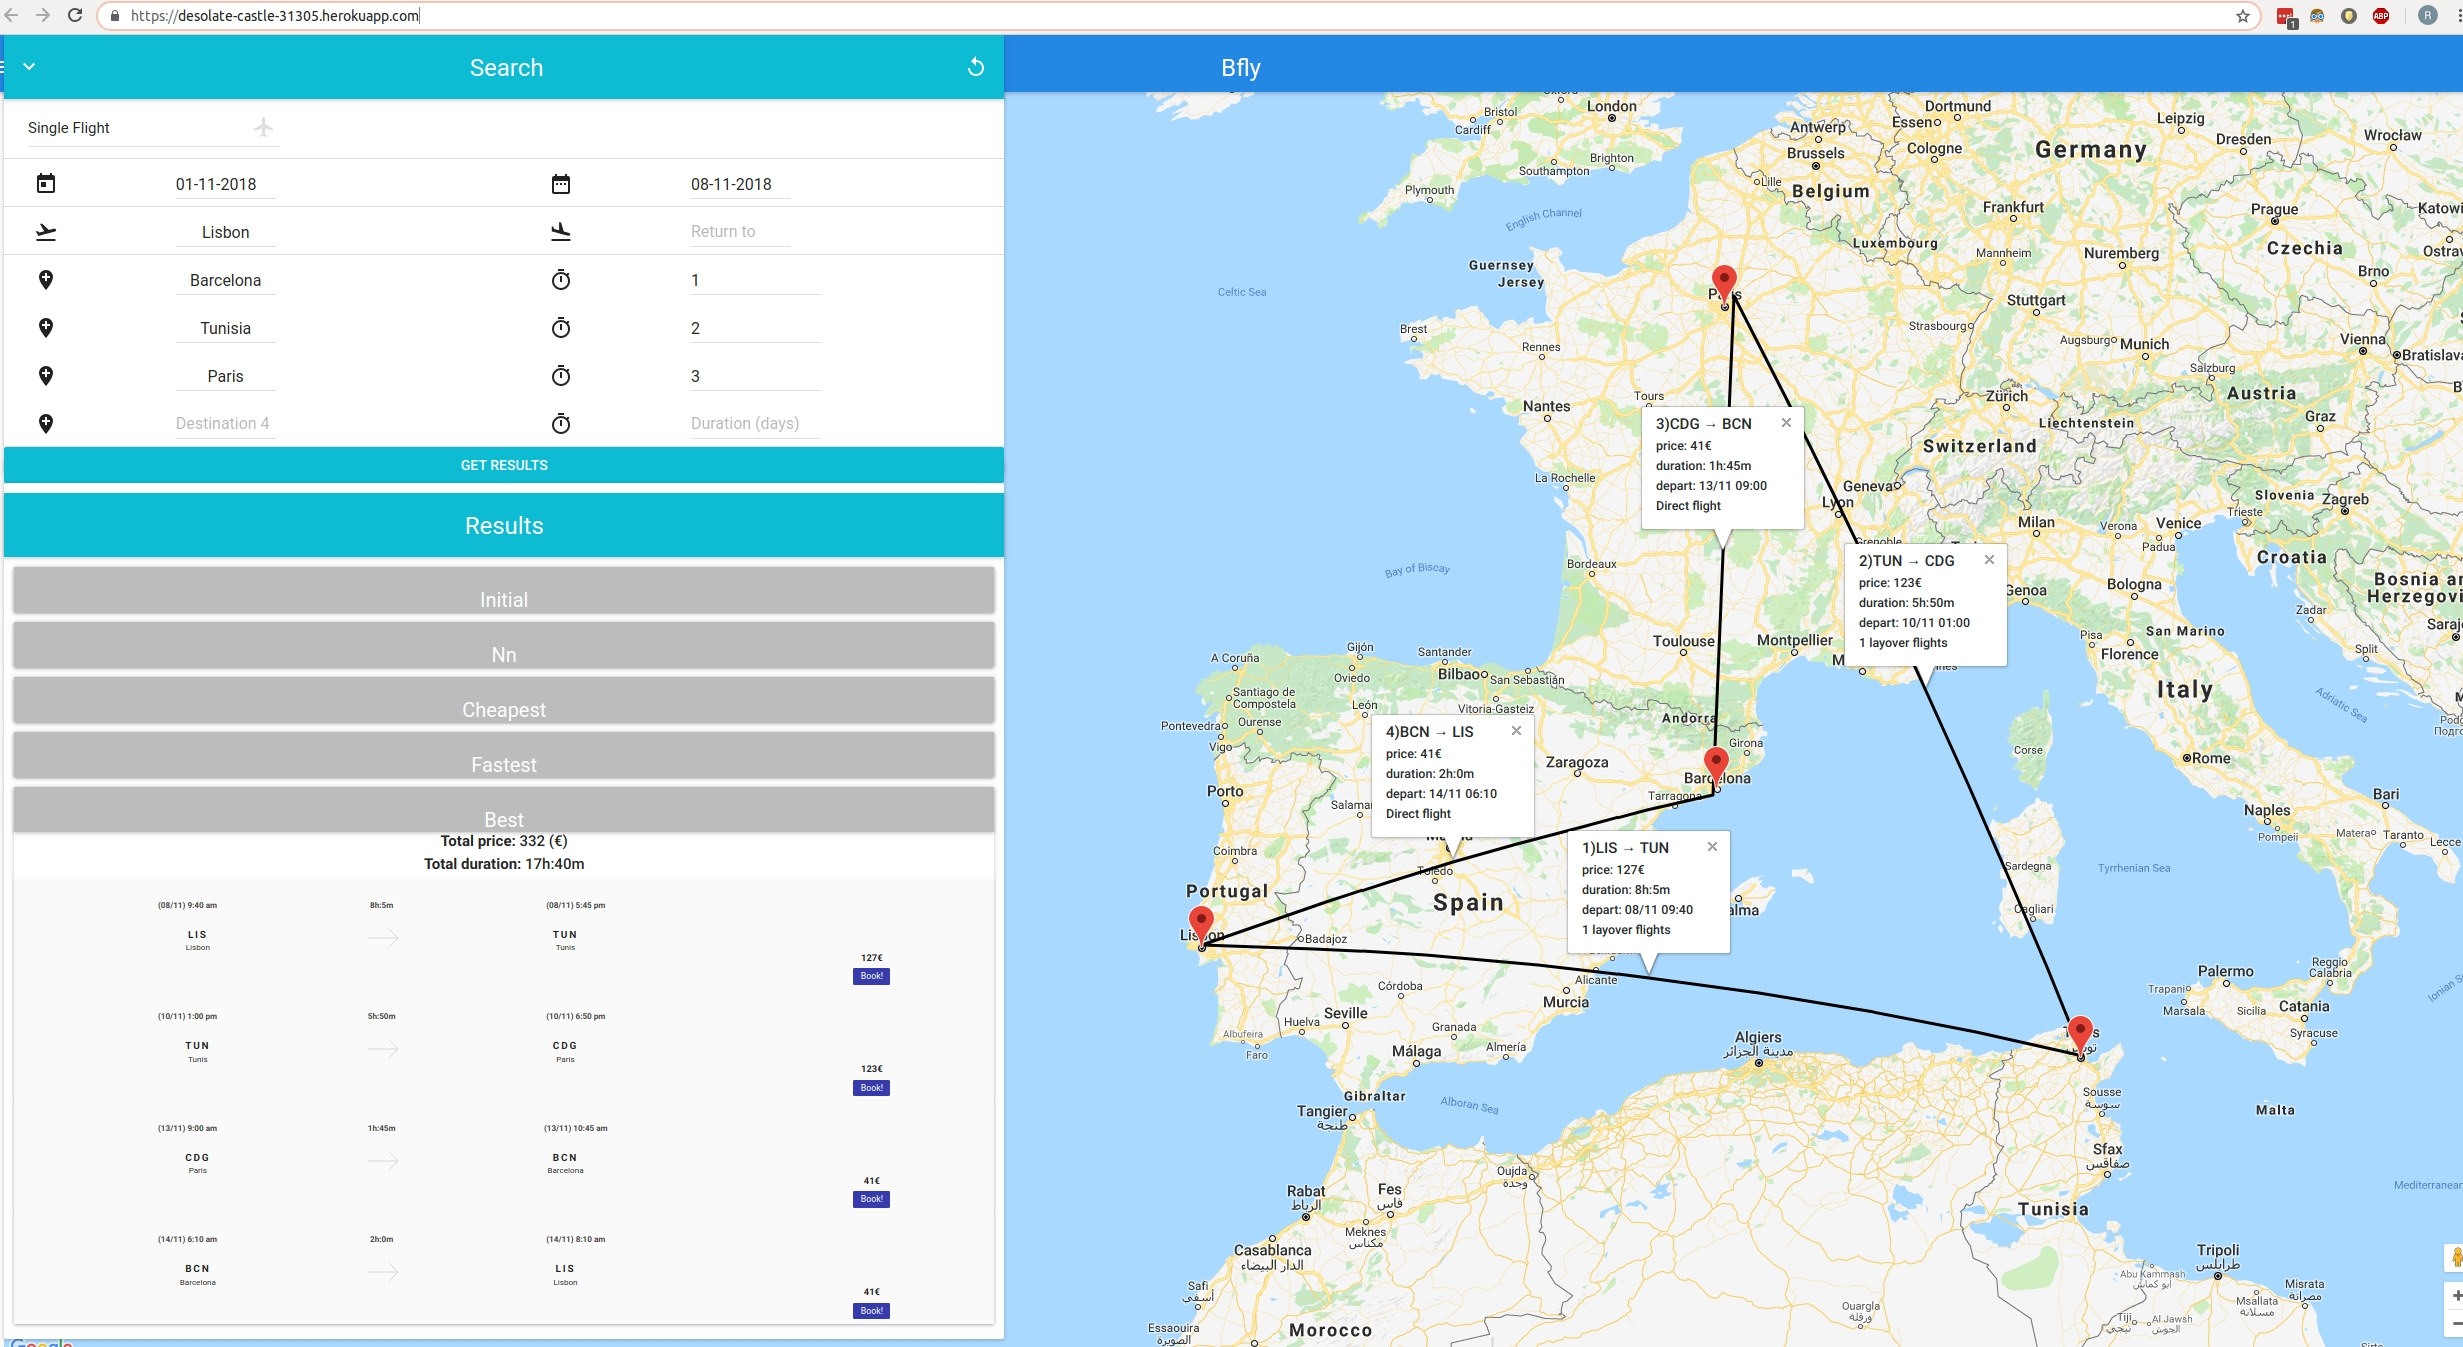
\includegraphics[width=\linewidth]{./imgs/bfly_desktop.jpg}
  \captionof{figure}{Application rendered on a desktop computer.}
  \label{fig:desktop_app}
\end{minipage}%
\begin{minipage}{.3\textwidth}
  \centering
  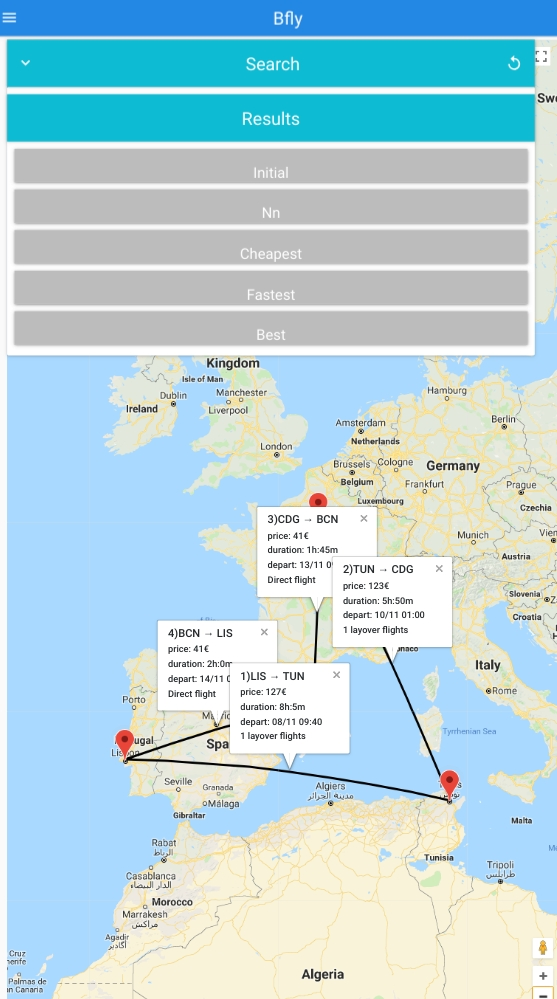
\includegraphics[width=0.75\linewidth]{./imgs/bfly_mobile.jpg}
  \captionof{figure}{Application rendered on a mobile device.}
  \label{fig:mobile_app}
\end{minipage}
\end{figure}

